\PassOptionsToPackage{hyphens}{url}
\documentclass[compress,aspectratio=169]{beamer}

\usetheme{Reading}

\graphicspath{{fig/}{img/}{../logo/}}

\newcommand{\ok}[1]{{#1 (done)}}
\newcommand{\ongoing}[1]{{#1 (ongoing)}}
\newcommand{\started}[1]{{#1 (started)}}
\newcommand{\pending}[1]{{#1 (pending in plan)}}
\newcommand{\hrefb}[2]{\href{#1}{\textcolor{blue}{#2}}}

\subtitle{}
\title{\huge Introducing the HPC Certification Program}
\author{J. Kunkel on behalf of the HPC Certification Forum}
\date{2018-10-31}
\authorURL{https://hpc-certification.org}
\authorFooter{Julian M. Kunkel}
\venue{Webinar}
\institute{Computer Science Department}
\groupLogo{
\includegraphics[width=2.5cm]{hpccf-small}}
\titleLogo{ 
\includegraphics[height=2.5cm]{blur-book-stack-books-590493}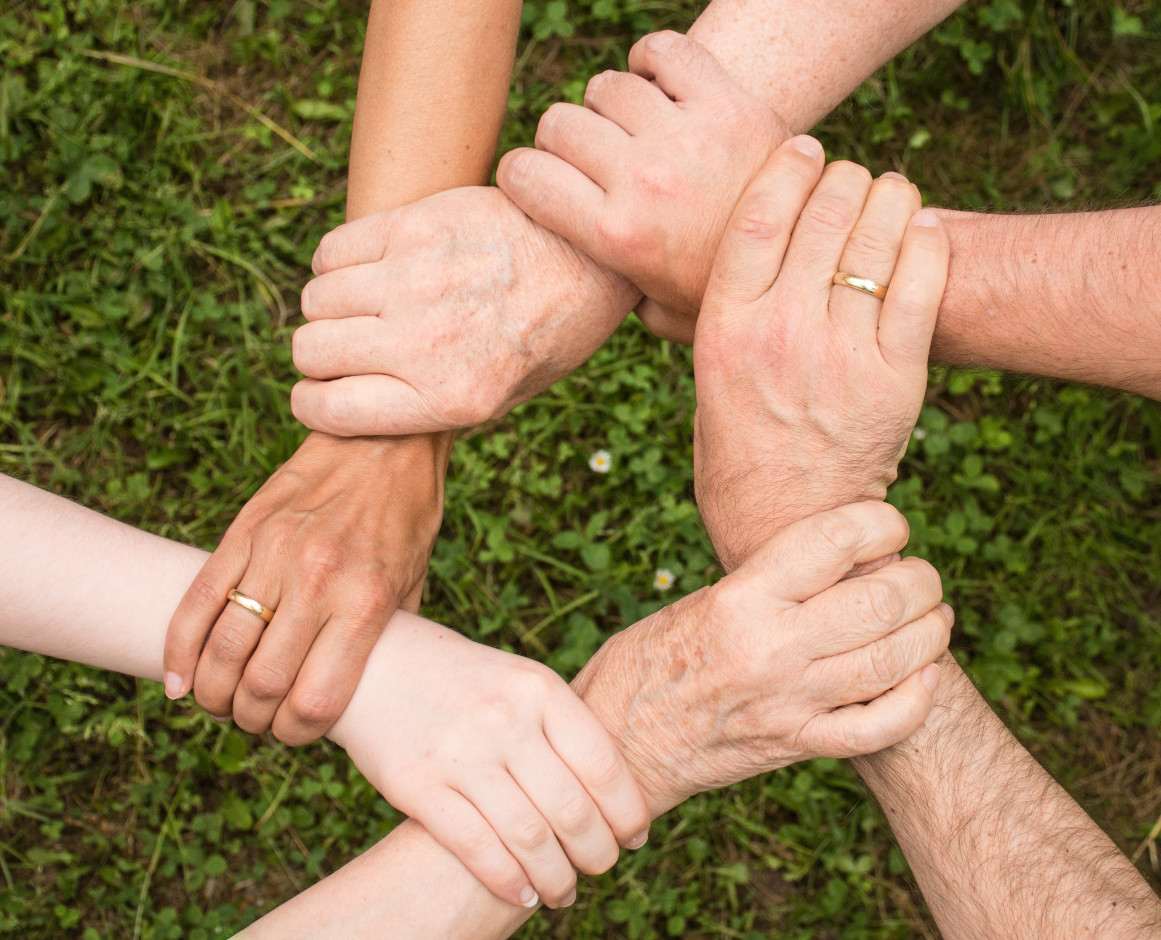
\includegraphics[height=2.5cm]{ground-group-growth-461049}
\includegraphics[height=2.5cm]{accomplishment-ceremony-college-267885}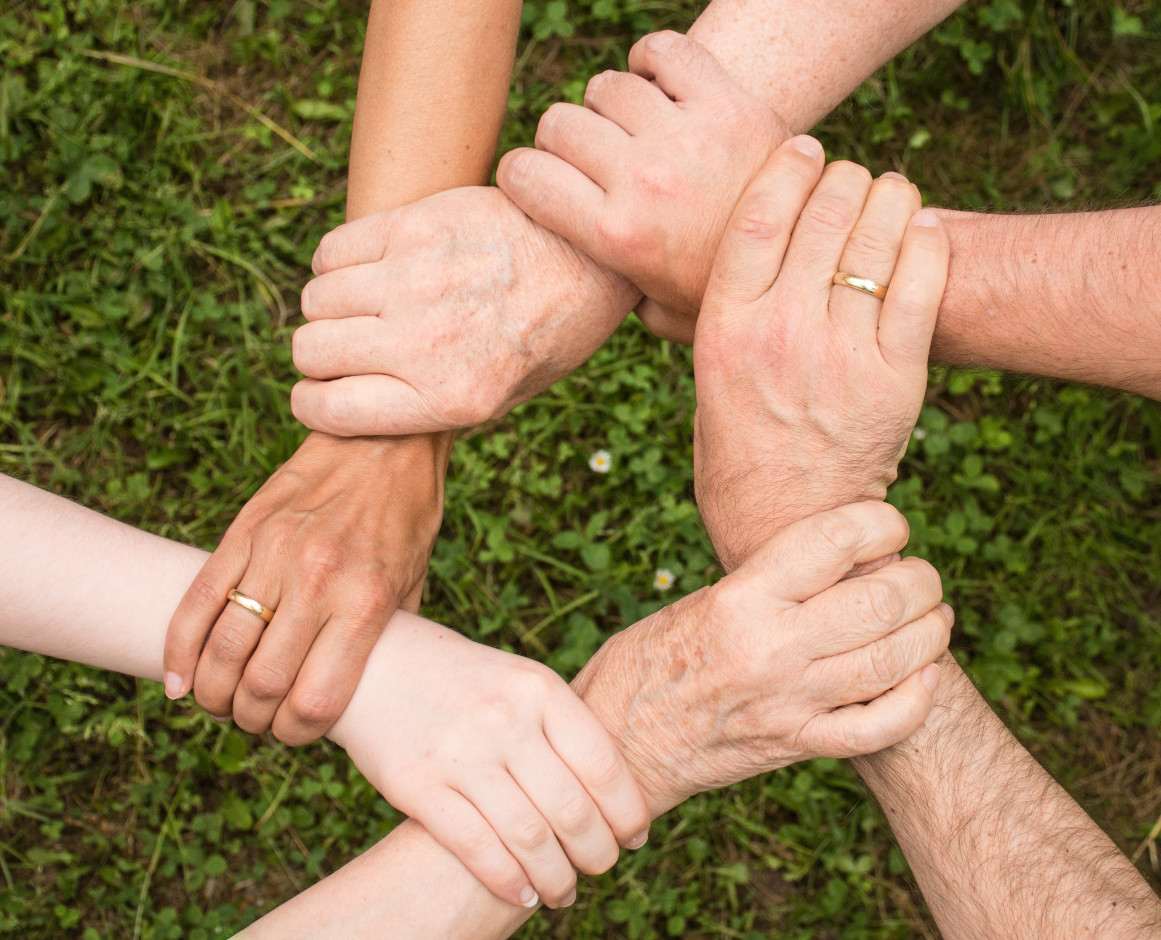
\includegraphics[height=2.5cm]{ground-group-growth-461049}
\includegraphics[height=2.5cm]{blur-book-stack-books-2}}


\begin{document}

\begin{frame}[plain]{}
	\maketitle
	{\fontsize{5.85pt}{6pt}\selectfont PeCoH is supported by Deutsche Forschungsgemeinschaft (DFG) under grants LU 1335/12-1, OL 241/2-1, RI 1068/7-1}
\end{frame}


% Title: Introducing the HPC Certification Program
% Abstract: This talk introduces the HPC Certification Forum and its
% activities to work towards an HPC certification program that will
% clearly categorize, define, and examine competencies for HPC
% practitioners.
% We will present the forum, concepts behind the program, the current
% status, and ongoing activities.
% Bio: Julian Kunkel is Lecturer in Computer Science at the University
% of Reading and managing the Performance Conscious HPC project which
% contributes to the HPC Certification Forum.
% He strongly believes that international recognition of skills will
% help the HPC ecosystem.




\section{The Program}
\sectionIntroHidden

\subsection{}

\begin{frame}{HPC Certification Program}
	\begin{block}{Motivation}
		\begin{itemize}

			\item Not all users possess the right level of training
				\begin{itemize}
				\item Inefficient usage of systems, frustration, lost potential
				\item Good training saves compute time and costs!
				\end{itemize}
			\item Learning is not easy
			\begin{itemize}
				\item Users need to understand beneficial knowledge for tasks
				\item Teaching of different data centers is hard to compare
			\end{itemize}
			\item Data center have difficulties to verify the skills of users
		\end{itemize}
	\end{block}

\end{frame}



\begin{frame}{The HPC Certification Program}
		\begin{block}{Goals}
			\begin{itemize}
				\item Standardizing HPC knowledge representation
          \begin{itemize}
            \item Supporting navigation and role-specific knowledge maps
          \end{itemize}
				\item Establishing international certificates attesting knowledge
			\end{itemize}
		\end{block}

    \textit{The work was bootstraped and is supported by the PeCoH project}
\end{frame}


\begin{frame}{Contributions by the PeCoH Project\footnote[frame]{PeCoH was supported by the German Research Foundation (DFG) under grants LU 1353/12-1, OL 241/2-1, and RI 1068/7-1.}}
	\begin{block}{Past contributions}
		\vspace*{-2mm}
		\begin{enumerate}
			\item Initial classification of competences
			\item Initial development of a certification program
		\end{enumerate}
	\end{block}

  The program will be curated by the 
\includegraphics[width=0.3\textwidth]{hpccf-full}

  \begin{block}{Pending contributions}
    \begin{itemize}
			\item Creation of workshop material for basic certificates
			\item Providing an online tutorial  for basic certificates
			\item Enabling an online examination
    \end{itemize}
  \end{block}
\end{frame}


\begin{frame}{Content of the Certification Program}
	\begin{itemize}
		\item Skill is characterized by unique key, background, knowledge covered
		\item Skill tree defining the organization of the competences
		\item Certificates bundle several skills into attestable unit
	\end{itemize}

		\begin{figure}
			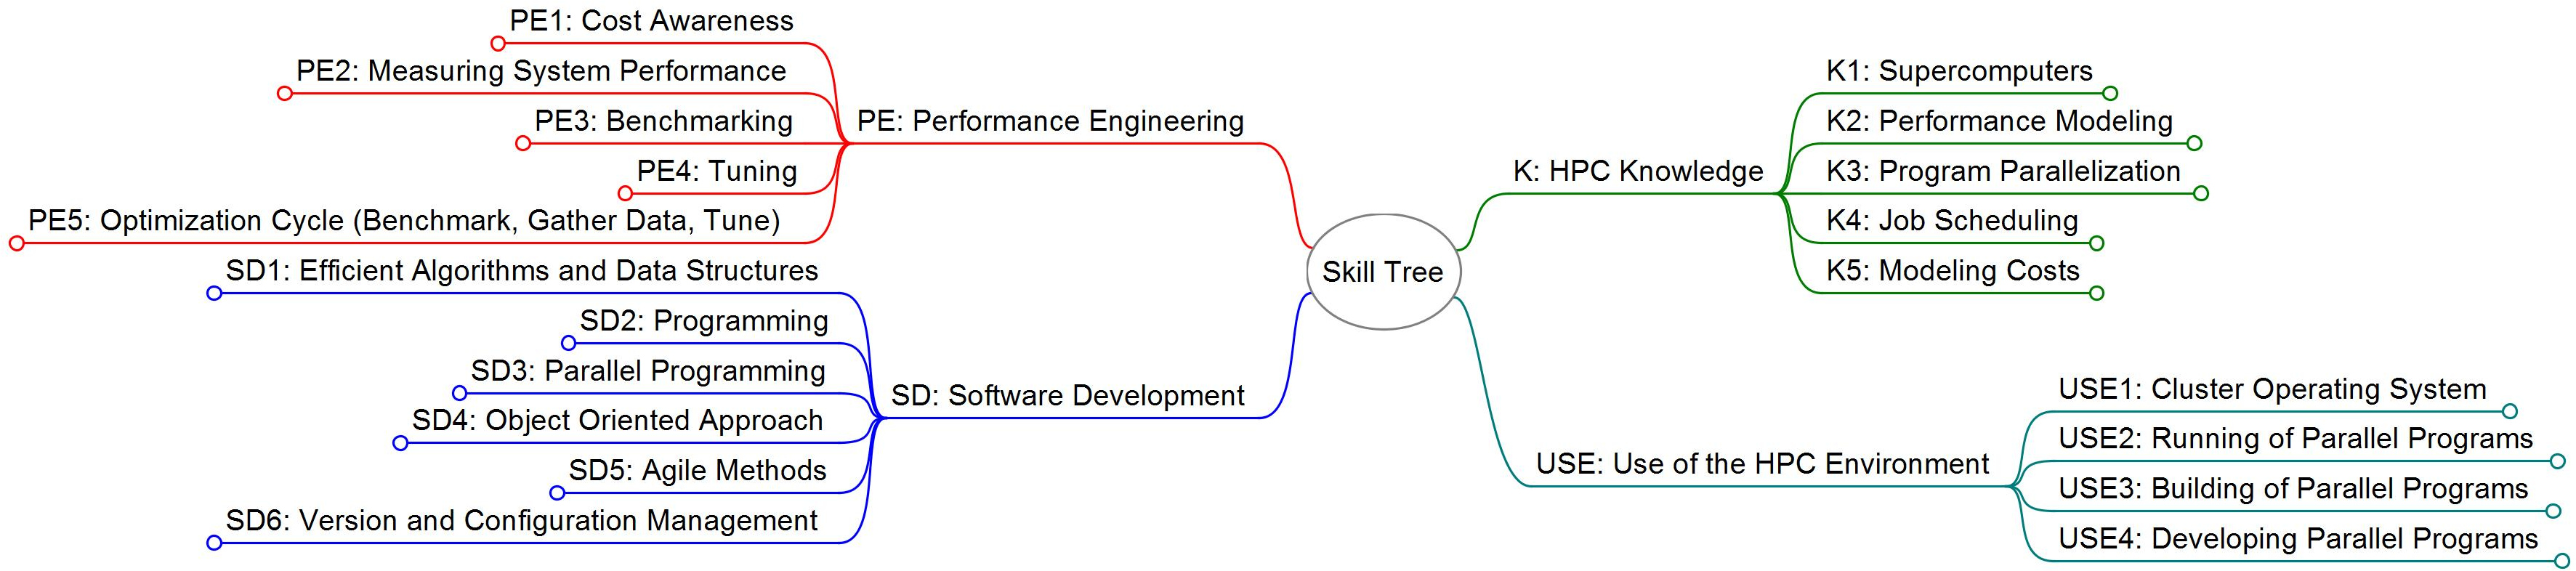
\includegraphics[width=\textwidth]{skill-tree_top_levels}
			\caption{Top-levels of the skill tree}
		\end{figure}

	\begin{itemize}
		\item Content is \textbf{NOT} covered and subject to content providers
		\begin{itemize}
			\item We may link good content on our page
		\end{itemize}
	\end{itemize}
\end{frame}


\begin{frame}{Example High-Level Skill}

	\begin{itemize}
		\item Name: Hardware Architectures
		\item Id: K1.2-B
		\item Level: Basic
		\item Category: HPC Knowledge
	\end{itemize}

	\begin{block}{Description of knowledge (aka what will the user learn)}
		\begin{itemize}
			\item Elementary processing elements like CPUs, GPUs, many core architectures
			\item Vector systems, and FPGAs
			\item The NUMA architecture used for symmetric multiprocessing
			\item Network demands for HPC systems (e.g. high bandwidth and low latency)
			\item Typical network architectures used for HPC systems, like fast Ethernet (1 or 10 Gbit) or InfiniBand
		\end{itemize}
	\end{block}
\end{frame}


\begin{frame}{Classification of HPC Competences}
	\begin{itemize}
		\item HPC skills are generally built upon one another
		\begin{itemize}
			\item Skills are typically depending on sub-skills $\Rightarrow$ tree structure
			\item References to skills are possible; still skills are building blocks for various tasks
		\end{itemize}
		\item Technical representation of the HPC skills
		\begin{itemize}
			\item Database for the HPC certification program
			\item Implementation is based on XML
			\item Corresponding XML Schema (XSD) assures consistency
		\end{itemize}

		\item Additional attributes are used to describe:
		\begin{itemize}
			\item Level of a skill (Basic, Intermediate, Expert)
			\item Suitability for a user role (Tester, Builder, Developer)
			\item Suitability for a scientific domain (Chemistry, Physics, ...)
		\end{itemize}
		\item Skill tree supports different views on the content
		\item \hrefb{https://www.hpc-certification.org/skills/}{Live Demo}
	\end{itemize}
\end{frame}




\begin{frame}{Status}
		\begin{block}{}
			\begin{itemize}
				\item A first version of the skill tree is released (35 basic skills)
					\begin{itemize}
						\item Technically implemented as XML
						\item Contribution is available on GitHub \\
							\url{https://github.com/HPC-certification-forum/curriculum}
					\end{itemize}
				\item JavaScript for visualization of skill tree
					\begin{itemize}
						\item Can be embedded in your webpage and adapted
							\begin{itemize}
								\item Role/software-specific knowledge
								\item What should people know to effectively work in your environment?
							\end{itemize}
					\end{itemize}
			\end{itemize}
		\end{block}
\end{frame}



\begin{frame}{Considerations}
	\begin{itemize}
		\item Granularity of skill descriptions
		\begin{itemize}
			\item Too fine $\Rightarrow$ content of a skill is predefined at leaf level
			\item Too coarse $\Rightarrow$ no help for structuring the material
			\item Actual skill tree contains 76 skills
		\end{itemize}

		\item Certificate definition
		\begin{itemize}
			\item Bundles a set of skills %(e.g. "Getting startet with HPC Clusters")
			\item A users' HPC qualification is certified by successful exams
		\end{itemize}
		\item Separation of skill, certificates and content provider
		\begin{itemize}
			\item Similar to the concept of a high school graduation exam %("Zentralabitur")
			\item Learning material can be provided by different institutions
			\item Teachers can put badges on material: this "trains XYZ"
		\end{itemize}
		\item Support flexible usage (views on skill tree) and skills is key
			\begin{itemize}
				\item Institutions can derive new skill tree with own groups \\
				e.g. users in weather/climate, single program, testers
				\item Realized via JavaScript (and JSON config files)
			\end{itemize}
	\end{itemize}
\end{frame}


\section{The HPC Certification Forum}
\sectionIntroHidden

\begin{frame}{The 
\includegraphics[width=0.45\textwidth]{hpccf-full}}
	The HPC-CF the central authority for the development of the program

	\begin{block}{Organization Details}
		\begin{itemize}
			\item An independent international body
			\item Organized into
				\begin{itemize}
					\item Steering board
					\item Full members with voting rights
					\item Associate members
				\end{itemize}
		\end{itemize}
	\end{block}

	\begin{block}{Responsibilities}
		\begin{itemize}
			\item Curating and maintaining the skill tree and certificates
			\item Providing tools and ecosystem around the competences
		\end{itemize}
	\end{block}
\end{frame}

\begin{frame}{Governance -- 2018}

  \begin{block}{Governance Rules}
    \vspace*{-0.3em}
    \begin{itemize}
      \item We have an initial set of governance rules
      \item Splitting responsibility across different roles
    \end{itemize}
  \end{block}

  \vspace*{-1em}

  \begin{block}{Current Chairs}
  \vspace*{-0.3em}
  \begin{itemize}
    \item Program chair: Julian Kunkel (University of Reading)
    \item Curriculum chair: Kai Himstedt (University of Hamburg)
    \item  Topic chairs:
    \begin{itemize}
      \item HPC Knowledge: Lev Lafayette (University of Melbourne)
      \item Performance Engineering: Anja Gerbes (University of Frankfurt)
      \item Use of the HPC Environment: Jean-Thomas Acquaviva (DDN)
      \item Software Development: \textit{Vacant, feel free to contact us}
    \end{itemize}
    \item Examination chair: not seated this year
    \item Publicity chair: Weronika Filinger
  \end{itemize}
  \end{block}
\end{frame}




\section{Conclusions \& Future Work}
\sectionIntroHidden

\begin{frame}{Outlook and Expected Benefits}
	\begin{block}{HPC practitioners}
		\vspace*{-0.2cm}
	\begin{itemize}
	\item Increase motivation to participate as the certificates are recognized in a CV
	\item Validate knowledge via tests
	\item Browse relevant competences
	\item Identify recommended and required skills related to certain tasks
	\item Understand and compare teaching offers across sites
	\end{itemize}
	\end{block}
	\vspace*{-0.3cm}
	\begin{block}{Data centers}
		\vspace*{-0.2cm}
	\begin{itemize}
	\item Increase sharing of teaching materials
	\item Simplifies documentation of taught skills
	\item Identify missing teaching activities
	\item Tailor skill-representation specifically to users
	\item Correlate lack of skills with efficient use
	\end{itemize}
	\end{block}
\end{frame}


\begin{frame}{Summary}

	\begin{block}{HPC Certification Program}
		\begin{itemize}
			\item Effort to standardize representation of relevant HPC skills
      \begin{itemize}
        \item Hierarchical definition of skills for practitioners
        \item Building blocks that can be cherry-picked for different tasks
      \end{itemize}
      \item It's goal is \textbf{NOT} to provide content or a linear curriculum
			\item Customizable navigation for compute centers
      \begin{itemize}
        \item Interactive viewer to browse skills and related content
      \end{itemize}
      \item Visit us and join our mailing lists: \url{https://hpc-certification.org}
		\end{itemize}
	\end{block}
\end{frame}

\begin{frame}{Next Steps}
		\begin{itemize}
			\item Finalizing the first version of the skill-tree (V1)
			\item Releasing the seal that can be added to training material
			\item Finalizing documentation how to create views with the JavaScript
        \begin{itemize}
          \item This will allow to outsource roles (e.g., tester) but also link to material
        \end{itemize}
      \item Creating a markdown version of the skill-tree (with converters)
      \item Embed a version that can be edited in an online Wiki (by members)
      \item Creation of workshop material and online certification (of base courses)
        \begin{itemize}
          \item Cheating has been a discussion, but we won't focus on this right now
        \end{itemize}
		\end{itemize}
  \label{frame:last}
\end{frame}




\end{document}
